
\documentclass[fleqn,12pt]{article}

\usepackage[margin=15mm]{geometry}
\usepackage[utf8]{inputenc}
\usepackage[bulgarian]{babel}
\usepackage[unicode]{hyperref}
\usepackage{amsfonts}
\usepackage{amssymb}
\usepackage{enumitem, hyperref}
\usepackage{upgreek}
\usepackage{indentfirst}
\usepackage{array}
\usepackage{listings}
\usepackage{xcolor}
\usepackage{csquotes}
\usepackage{dirtytalk}
\usepackage{graphicx}

\usepackage{amsmath}
\DeclareMathOperator{\cotg}{cotg}
\DeclareMathOperator{\LCS}{LCS}
\DeclareMathOperator{\longer}{longer}

\definecolor{codegreen}{rgb}{0,0.6,0}
\definecolor{codegray}{rgb}{0.5,0.5,0.5}
\definecolor{codepurple}{rgb}{0.58,0,0.82}
\definecolor{backcolour}{rgb}{0.95,0.95,0.92}

\lstdefinestyle{mystyle}{
    backgroundcolor=\color{backcolour},   
    commentstyle=\color{codegreen},
    keywordstyle=\color{magenta},
    numberstyle=\tiny\color{codegray},
    stringstyle=\color{codepurple},
    basicstyle=\ttfamily\footnotesize,
    breakatwhitespace=false,
    breaklines=true,
    captionpos=b,
    keepspaces=true,
    numbers=left,
    numbersep=5pt,
    showspaces=false,
    showstringspaces=false,
    showtabs=false,
    tabsize=2,
    inputencoding=utf8,
    extendedchars=true,
    literate={а}{\cyra}1
    {б}{{\selectfont\char225}}1
    {в}{{\selectfont\char226}}1
    {г}{{\selectfont\char227}}1
    {д}{{\selectfont\char228}}1
    {е}{{\selectfont\char229}}1
    {ё}{{\"e}}1
    {ж}{{\selectfont\char230}}1
    {з}{{\selectfont\char231}}1
    {и}{{\selectfont\char232}}1
    {й}{{\selectfont\char233}}1
    {к}{{\selectfont\char234}}1
    {л}{{\selectfont\char235}}1
    {м}{{\selectfont\char236}}1
    {н}{{\selectfont\char237}}1
    {о}{{\selectfont\char238}}1
    {п}{{\selectfont\char239}}1
    {р}{{\selectfont\char240}}1
    {с}{{\selectfont\char241}}1
    {т}{{\selectfont\char242}}1
    {у}{{\selectfont\char243}}1
    {ф}{{\selectfont\char244}}1
    {х}{{\selectfont\char245}}1
    {ц}{{\selectfont\char246}}1
    {ч}{{\selectfont\char247}}1
    {ш}{{\selectfont\char248}}1
    {щ}{{\selectfont\char249}}1
    {ъ}{{\selectfont\char250}}1
    {ы}{{\selectfont\char251}}1
    {ь}{{\selectfont\char252}}1
    {э}{{\selectfont\char253}}1
    {ю}{{\selectfont\char254}}1
    {я}{{\selectfont\char255}}1
    {А}{{\selectfont\char192}}1
    {Б}{{\selectfont\char193}}1
    {В}{{\selectfont\char194}}1
    {Г}{{\selectfont\char195}}1
    {Д}{{\selectfont\char196}}1
    {Е}{{\selectfont\char197}}1
    {Ё}{{\"E}}1
    {Ж}{{\selectfont\char198}}1
    {З}{{\selectfont\char199}}1
    {И}{{\selectfont\char200}}1
    {Й}{{\selectfont\char201}}1
    {К}{{\selectfont\char202}}1
    {Л}{{\selectfont\char203}}1
    {М}{{\selectfont\char204}}1
    {Н}{{\selectfont\char205}}1
    {О}{{\selectfont\char206}}1
    {П}{{\selectfont\char207}}1
    {Р}{{\selectfont\char208}}1
    {С}{{\selectfont\char209}}1
    {Т}{{\selectfont\char210}}1
    {У}{{\selectfont\char211}}1
    {Ф}{{\selectfont\char212}}1
    {Х}{{\selectfont\char213}}1
    {Ц}{{\selectfont\char214}}1
    {Ч}{{\selectfont\char215}}1
    {Ш}{{\selectfont\char216}}1
    {Щ}{{\selectfont\char217}}1
    {Ъ}{{\selectfont\char218}}1
    {Ы}{{\selectfont\char219}}1
    {Ь}{{\selectfont\char220}}1
    {Э}{{\selectfont\char221}}1
    {Ю}{{\selectfont\char222}}1
    {Я}{{\selectfont\char223}}1
}
\lstset{style=mystyle}

\graphicspath{ {./img/} }

\title{Морфологическа реконструкция на изображения}

\begin{document}

\maketitle
\begin{center}
\textbf{Иван Христов Христов, Ф№ 2MI3400066, Специалност - Изкуствен Интелект}

\tableofcontents

\end{center}

\section{Неформална дефиниция}

\textbf{\textit{Морфологическата реконструкция}} е техника за изграждане на изображение от малки компоненти или извличане на компоненти от изображение без нарушаване на тяхната цялост. Приложима е над двоични и полутонови изображения. Обичайно алгоритмите прилагащи морф. операции приемат като вход оригинално изображение и структурен елемент, който да приложат над него. За разлика от тях \textit{морф. реконструкция} приема като вход 3 аргумента:
\begin{enumerate}
    \item \textit{\textbf{маска}} - оригиналното изображение, ограничаващо трансформацията, от което искаме да извлечем компонентите,
    \item \textit{\textbf{маркер}} - изображение, съдържащо стартовите точки на трансформацията,
    \item \textit{\textbf{ядро/структурен елемент}} - дефинира свързаността (4-свързаност, 8-свързаност и т.н.) при прилагане на морф. операции като дилация и ерозия.
\end{enumerate}

Изходът от операцията е изображение, което съдържа подмножество от компонентите на оригиналното изображение.

\bigbreak

В зависимост от това, което искаме да постигнем можем да приложим различна имплементация. Разновидности се постигат са чрез:
\begin{itemize}
    \item \textit{дилация} - за извличане на светли части и обекти от маски,
    \item \textit{ерозия} - за извличане на тъмни части и дупки на обекти от маски,
    \item \textit{трансформация по разстояние (distance transform)} - за извличане на обекти с конкретни дебелини.
\end{itemize}

Ние ще се фокусираме над дилация и ерозия.

\section{Формални дефиниции}

Нека приемем, че маската ни е $X$, маркера - $Y$, $B$ - ядрото и $Z$ - търсеното изображение. Най-често морф. реконструкция дефинираме чрез термина геодезично разстояние.

\bigbreak

\textit{\textbf{Деф}} - Нека $F \subset \mathbb{Z}^2$ е изображение. Геодезично разстояние между два пиксела $p$ и $q$ от $F$ дефинираме като дължината най-краткия път $path$ между $p$ и $q$, където $\forall r \in path$ $r \in F$. Означаваме го чрез $d_F (p, q)$.

\bigbreak

\textit{\textbf{Деф}} - Нека $F, Y \subset \mathbb{Z}^2$ са изображения и $Y \subseteq F$. Геодезичното разстояние между пиксел $p \in F$ и $Y$ дефинираме като $d_F (p, Y) = min\{d_F (p, q) | q \in Y\}$.

\bigbreak

Съответно можем да дефинираме термина "геодезична дилация":

\textit{\textbf{Деф}} - Нека $X, Y \in \mathbb{Z}^2$ и $Y \subseteq X$. \textbf{\textit{Геодезична дилация}} от размер $n \geq 0$ на $Y$ от $X$ се дефинира като множеството от пиксели на $X$ с геодезично разстояние по-малко или равно на $n$ до $Y$, т.е.:

\begin{center}
    $\delta_X^{(n)} (Y) = \{p \in X | d_X (p, Y) \leq n\}$. 
\end{center}


\bigbreak

\textit{\textbf{Заб}} - $Y \subseteq \delta_X^{(n)} (Y)$.

\bigbreak

\textit{\textbf{Заб}} - Геодезична дилация от размер $n$ може да се разглежда като резултата от прилагане на геодезична дилация от размер $1$ $n$ пъти:

$$
    \delta_X^{(n)} (Y) = \underbrace{\delta_X^{(1)} \circ \delta_X^{(1)} \circ \dots \circ \delta_X^{(1)} (Y)}_{n\ times}
$$

\textit{\textbf{Деф}} - Геодезична дилация от размер 1 наричаме елементарна геодезична дилация.

\bigbreak

\textit{\textbf{Тв}} - $\delta_X^{(1)} (Y) = (Y \oplus B) \cap X$, където $B$ е ядро определящо свързаността. Доказателството оставяме като упражнение за читателя.

\bigbreak

\textit{\textbf{Деф}} - Реконструкция базирана на дилация за бинарни изображения на маркер $Y$ от маска $X$, където $Y \subseteq X$ получаваме чрез последователно прилагане на елементарни геодезични дилации до стигане на сходство:
$$\rho_X^\delta (Y) = \bigcup_{i=1}^{n} \delta_X^{(n)} (Y)$$, където $\delta_X^{(n)} (Y) = \delta_X^{(n + 1)} (Y)$.

\bigbreak

По сходен начин можем да дефинираме и реконструкция чрез ерозия.

\textit{\textbf{Деф}} - Нека $X, Y \subset \mathbb{Z}^2$ и $X \subseteq Y$. \textit{\textbf{Геодезична ерозия}} от размер $n \geq 0$ на $Y$ от $X$ се дефинира като множеството от пиксели на $Y$ с геодезично разстояние по-голямо или равно на $n$ до $X \setminus Y$:

$$\varepsilon_X^{(n)} (Y) = \{p \in Y | d_X(p, X \setminus Y) \geq n\}$$.

\bigbreak

\textit{\textbf{Заб}} - $\varepsilon_X^{(n)} (Y)  \subseteq Y$.

\bigbreak

\textit{\textbf{Деф}} - Геодезична ерозия от размер $n$ може да се разглежда като резултата от прилагане на геодезична ерозия от размер $1$ $n$ пъти:

$$
    \varepsilon_X^{(n)} (Y) = \underbrace{\varepsilon_X^{(1)} \circ \varepsilon_X^{(1)} \circ \dots \circ \varepsilon_X^{(1)} (Y)}_{n\ times}
$$

\bigbreak

\textit{\textbf{Тв}} - $\varepsilon_X^{(1)} (Y) = (Y \ominus B) \cup X$, където $B$ е ядро определящо свързаността. Доказателството оставяме като упражнение за читателя.

\bigbreak

\textit{\textbf{Деф}} - Геодезична ерозия от размер 1 наричаме елементарна геодезична ерозия.

\bigbreak

\textit{\textbf{Деф}} - Реконструкция базирана на ерозия за бинарни изображения на маркер $Y$ от маска $X$, където $X \subseteq Y$ получаваме чрез последователно прилагане на елементарни геодезични ерозии до стигане на сходство:
$$\rho_X^\varepsilon (Y) = \bigcap_{i=1}^{n} \varepsilon_X^{(n)} (Y)$$, където $\varepsilon_X^{(n)} (Y) = \varepsilon_X^{(n+1)} (Y)$.

\section{Алгоритми за реконструкция на бинарни изображения}

\subsection{Чрез дилация}

Маркерът съдържа компоненти, които са подмножества на други компоненти от маската. Обичайно това са само точки. С други думи $Y \subseteq X$. Изходът от операцията е изображение, което съдържа компонентите от оригиналното изображение, за които сме посочили подмножество в маркера. Обичайно като структурен елемент се задава, т.е. ползваме 8-свързаност:

\begin{equation}
    B = \begin{pmatrix}
    1 & 1 & 1 \\
    1 & 1 & 1 \\
    1 & 1 & 1
    \end{pmatrix}
\end{equation}

Алгоритъма за реконструкция чрез дилация може да се сведе до:
\begin{enumerate}
    \item Нека $h_1 = g$.
    \item $h_{i+1} = (h_{i} \oplus B) \cap f$.
    \item Ако $h_{i+1} = h_i$, то $h = h_{i+1}$ и алгоритъмът приключва. В противен случай се връщаме към 2. Имаме гаранция, че алгоритъмът ще приключи защото маската ограничава изходното изображение.
\end{enumerate}

\subsubsection{Пример}

\begin{lstlisting}[caption=Example for reconstruction based on dilation]
// mask             // marker           // after step 1     // after step 2
0 0 0 0 0 0 0 0     0 0 0 0 0 0 0 0     0 0 0 0 0 0 0 0     0 0 0 0 0 0 0 0
0 0 0 0 0 0 0 0     0 0 0 0 0 0 0 0     0 0 0 0 0 0 0 0     0 0 0 0 0 0 0 0
0 0 1 0 0 0 0 0     0 0 1 0 0 0 0 0     0 0 1 0 0 0 0 0     0 0 1 0 0 0 0 0 
0 0 1 1 1 0 0 0     0 0 0 0 0 0 0 0     0 0 1 1 0 0 0 0     0 0 1 1 1 0 0 0
0 0 1 0 1 0 0 0     0 0 0 0 0 0 0 0     0 0 0 0 0 0 0 0     0 0 1 0 1 0 0 0
0 0 0 0 0 0 0 0     0 0 0 0 0 0 0 0     0 0 0 0 0 0 0 0     0 0 0 0 0 0 0 0
0 0 0 0 0 0 0 0     0 0 0 0 0 0 0 0     0 0 0 0 0 0 0 0     0 0 0 0 0 0 0 0
0 0 1 1 0 0 0 0     0 0 0 0 0 0 0 0     0 0 0 0 0 0 0 0     0 0 0 0 0 0 0 0
\end{lstlisting}


\begin{figure}
    \centering
    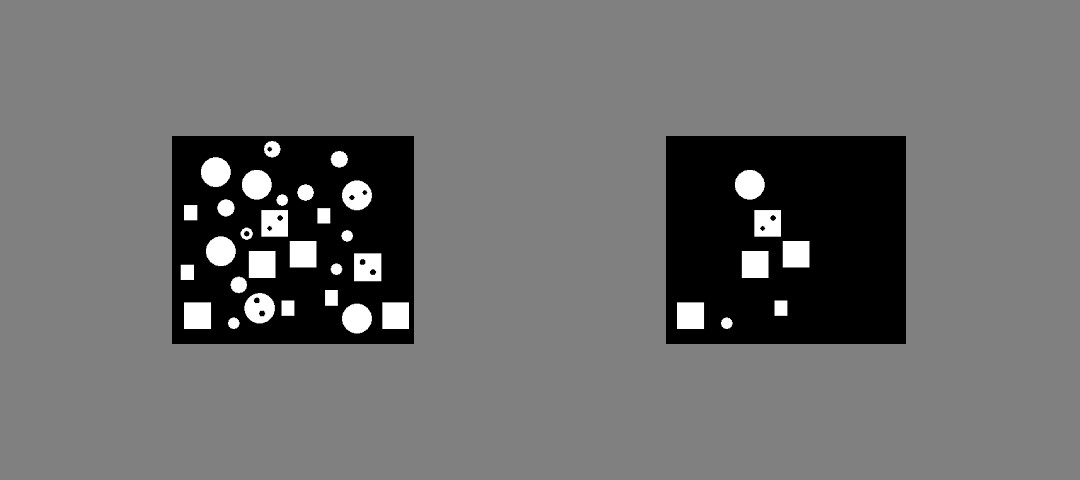
\includegraphics[width=\textwidth]{img/dil_rec.jpg}
    \caption{Реконструкция на бинарно изображение чрез дилация}
    \label{fig:dil_rec}
\end{figure}


\subsection{Реконструкция чрез ерозия}

Маската е подмножество на маркера, т.е. $X \subseteq Y$. Изходът от операцията е изображение, което съдържа тъмни петна или дупки от оригиналното изображение. Отново ще използваме 8-свързаност. Алгоритъмът за реконструкция чрез ерозия може да се сведе до:
\begin{enumerate}
    \item Нека $h_1 = g$.
    \item $h_{i+1} = (h_{i} \ominus B) \cup f$.
    \item Ако $h_{i+1} = h_i$, то $h = h_{i+1}$ и алгоритъмът приключва. В противен случай се връщаме към 2. Имаме гаранция, че алгоритъмът ще приключи защото маската ограничава изходното изображение.
\end{enumerate}

\subsubsection{Пример}

\begin{lstlisting}[caption=Example for reconstruction based on dilation]
// mask             // marker           // after step 1     // after step 2
0 0 0 0 0 0 0 0     0 0 0 0 0 0 0 0     0 0 0 0 0 0 0 0     0 0 0 0 0 0 0 0
0 0 0 0 0 0 0 0     0 0 0 0 0 0 0 0     0 0 0 0 0 0 0 0     0 0 0 0 0 0 0 0
0 0 1 0 0 0 0 0     0 0 1 0 0 0 0 0     0 0 1 0 0 0 0 0     0 0 1 0 0 0 0 0 
0 0 1 1 1 0 0 0     0 0 1 1 1 0 0 0     0 0 1 1 1 0 0 0     0 0 1 1 1 0 0 0
0 0 1 0 1 0 0 0     0 0 1 1 1 0 0 0     0 0 1 1 1 0 0 0     0 0 1 0 1 0 0 0
0 0 1 0 1 0 0 0     0 0 1 1 1 0 0 0     0 0 1 0 1 0 0 0     0 0 1 0 1 0 0 0
0 0 1 0 1 0 0 0     0 0 1 0 1 0 0 0     0 0 1 0 1 0 0 0     0 0 1 0 1 0 0 0
0 0 1 1 1 0 0 0     0 0 1 1 1 0 0 0     0 0 1 1 1 0 0 0     0 0 1 1 1 0 0 0
\end{lstlisting}

\begin{figure}
    \centering
    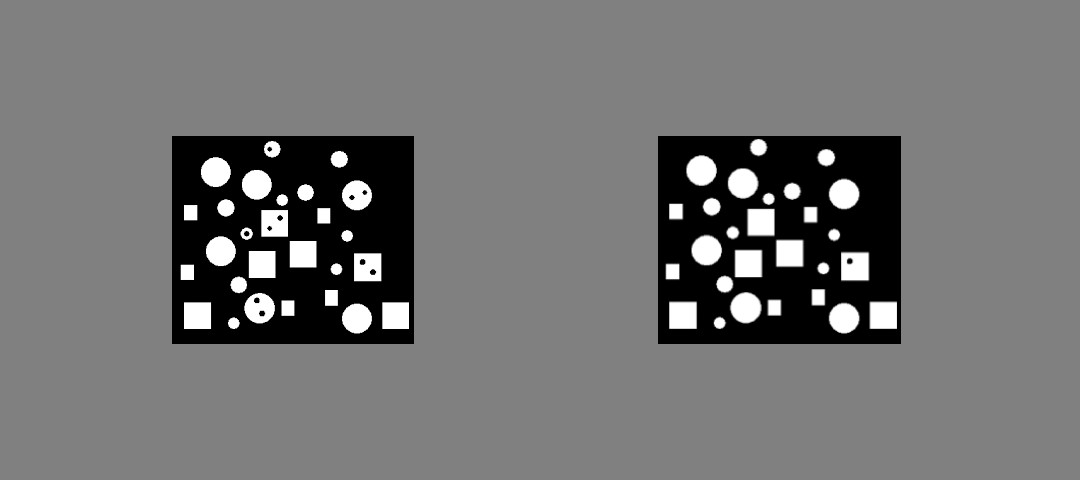
\includegraphics[width=\textwidth]{img/er_rec.jpg}
    \caption{Реконструкция на бинарно изображение чрез ерозия}
    \label{fig:er_rec}
\end{figure}

\section{Реконструкция на полутонови изображения}

\begin{figure}
    \centering
    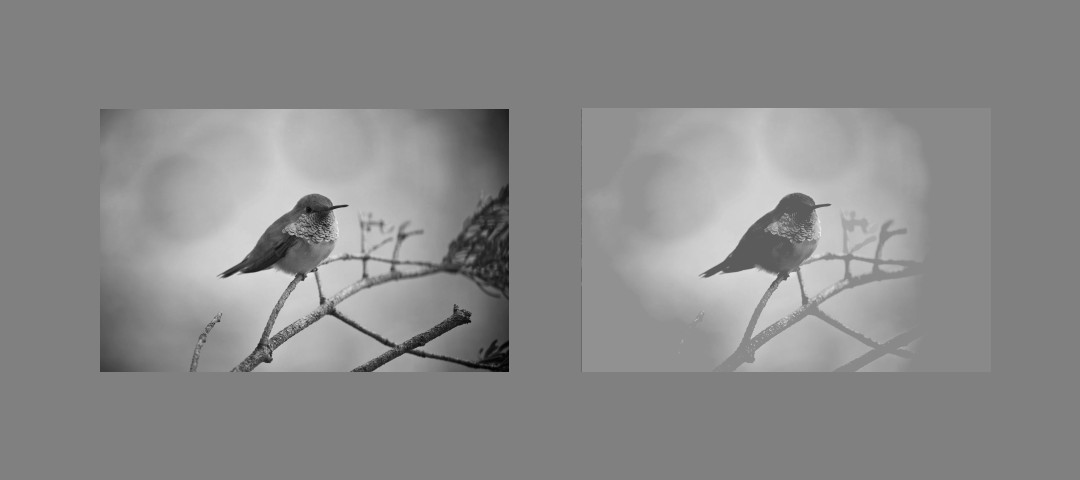
\includegraphics[width=\textwidth]{img/grayscale_rec.jpg}
    \caption{Реконструкция на полутоново изображение чрез ерозия}
    \label{fig:g_er_rec}
\end{figure}

\textbf{\textit{Деф}} - Нека имаме нива на интензитета $\{0, 1, \dots, N-1\}$ и имаме изображение $X$. Тогава дефинираме:
$$T_k(I) = \{p \in X | I(p) \geq k\}$$.

\bigbreak

\textbf{\textit{Деф}} - \textit{\textbf{Прагова декомпозиция}} наричаме $T(I) = \{T_k(I) | k \in \{0, 1, \dots, N-1\}\}$.

\bigbreak

Забелязваме, че всяка нарастваща морф. операция $\psi$ в някое изображение $X$ е изпълнено:
$$\forall p \in X, \psi(I)(p) = max\{k \in \{0, 1, \dots, N-1\} | p \in \psi(T_k(I))\}$$.

\bigbreak \textbf{\textit{Заб}} - Морф. реконструкция е нарастваща операция. Следователно морф. реконструкция за полутонови изображения можем да дефинираме по следния начин:

\bigbreak

\textbf{\textit{Деф}} - Нека $Y$ (маркер) и $X$ (маска) са полутонови изображения, поемащи интензитет от $\{0, \dots, N-1\}$ и такива, че $Y \leq X$. Полутонова морф. реконструкция чрез дилация $\rho_X^\delta (Y)$ от $X$ дефинираме като:

$$\forall p \in X, \rho_X^\delta (Y)(p) = max\{k \in \{0, \dots, N-1\} | p \in \rho_{T_k(X)}^\delta (T_k(Y))\}$$.

\bigbreak

За пояснение разделяме изображението на няколко нива, като имаме по едно ниво за всяка стойност на интензитета. След това третираме всеки слой като бинарно изображение и накрая взимаме максималната стойност от всички слоеве за конкретния пиксел. Това обаче е много бавно за имплементация и може да се запише по по-удобен начин.

\bigbreak

\textbf{\textit{Деф}} - Елементарна полутонова геодезична дилация над изображение $X$ с маркер $Y$ дефинираме като:
$$\delta_X^{(1)} (Y) = (Y \oplus B) \land X$$, където $\land$ е точков оператор за минимум.

\bigbreak

\textbf{\textit{Тв}} - Може да се докаже, че:

$$ \rho_X^\delta (Y) = \bigvee\limits_{n \geq 1} \delta_X^{(n)} (Y)$$.

\bigbreak

На интутивно ниво начина, по който прилагаме морф. реконструкция чрез дилация, върху полутонови изображения резултира в отрязване компоненти, които са под конкретна стойност на интензитета зададена в маркера.

\bigbreak

По сходен начин може да се приложи и ерозия върху много нива, но тя работи в обратната посока. Полутонова геодезична ерозия се прилага за изрязване на тепета на компоненти от изображения.

\bigbreak

\textbf{\textit{Деф}} - Елементарна полутонова геодезична ерозия над изображение $X$ с маркер $Y$ дефинираме като:
$$\varepsilon_X^{(1)} (Y) = (Y \ominus B) \lor X$$, където $\lor$ е точков оператор за максимум.

\bigbreak

\textbf{\textit{Тв}} - Може да се докаже, че:

$$ \rho_X^\varepsilon (Y) = \bigwedge\limits_{n \geq 1} \varepsilon_X^{(n)} (Y)$$.


\section{Реконструкция на цветни изображения}

Възможно е по заобиколен път да се приложи реконструкция и върху цветни изображения. Това е лично моя измишльотина и го направих по следния начин:

\begin{enumerate}
    \item Използвам Гаусов филтър за да замажа изображението.
    \item Конвертирам изображението към полутоново, запазвайки оригиналното такова.
    \item Изравнявам хистограмата за да получа по-добър контраст.
    \item Филтрирам по Лаплас, като прилагам втора производна за да намеря ръбовете на обектите от изображението. Оставям контурите да са бели, а фона черен.
    \item Бинаризирам изображението.
    \item Използвам реконструкция чрез ерозия върху бинарното изображение за да намеря участъците.
    \item Прилагам поточков минимум между реконструираното изображение и оригинала.
\end{enumerate}

Получените резултати не са най-добрите възможни, но показват, че може по някакъв начин този метод да се приложи и върху цветни изображения.

\begin{figure}
    \centering
    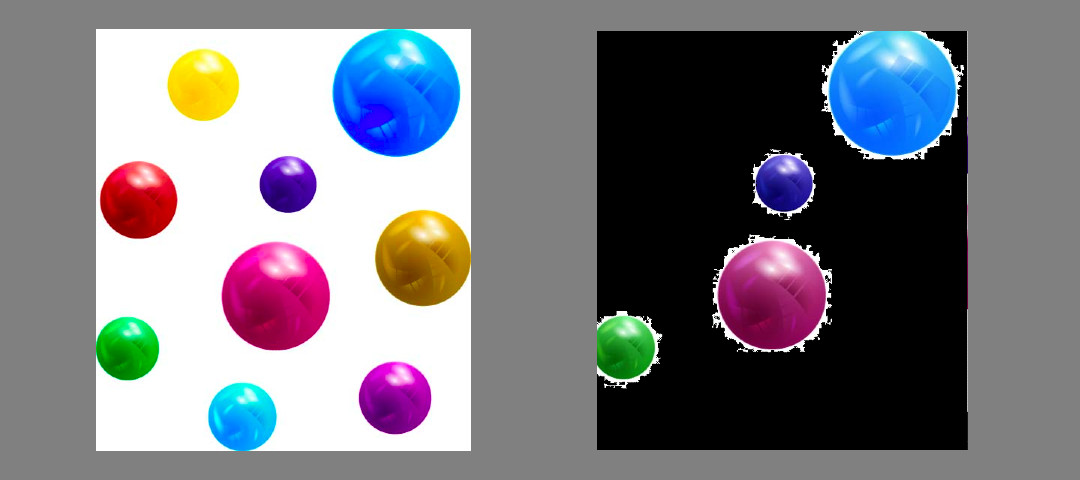
\includegraphics[width=\textwidth]{img/col_rec.jpg}
    \caption{Реконструкция на цветно изображение}
    \label{fig:col_rec}
\end{figure}


\section{Ресурси}

\begin{itemize}
    \item http://www.vincent-net.com/luc/papers/93ieeeip\_recons.pdf
    \item https://www.youtube.com/watch?v=MFDAq09s1e4
    \item https://zone.ni.com/reference/en-XX/help/372916T-01/nivisionconcepts/morphological\_reconstruction/
\end{itemize}

\end{document}
